\section{Introduction}
\label{sec:introduction}

In this laboratory, we analysed in a theoretical approach as well as using software simulation, an Amplifier made of Bipolar Junction Transistors.
It was composed of two different stages: a Gain Stage (with the objective of having the maximum gain possible, as we'll discuss in greater detail) and an Output Stage (whose objective is to lower the impedance of the Amplifier, to allow a better connection to the Load). In this report, a software simulation and theoretical analysis will be stacked up against each other. This assignment allowed us to deal with important concepts such as \textbf{BJTs Transistors} and its diverse utility in circuits. In Figure \ref{fig:circuitol3} the stated circuit is presented. 

A theoretical analysis of the circuit will be presented combining Operating Point (DC), which allows us to derive important values for the incremental analysis (AC). 
Also, regarding BJTs it is important to notice that there were used two different models, both of them by Philips: BC557A (PNP) and BC547A (NPN).  

Simultaneously, the circuit is analysed by computational simulation tools, via \textit{Ngspice}, and the results are compared to the theoretical results obtained, in Section \ref{sec:analysis}. The conclusions of this study are outlined in Section \ref{sec:conclusion}.

\begin{figure}[h] \centering
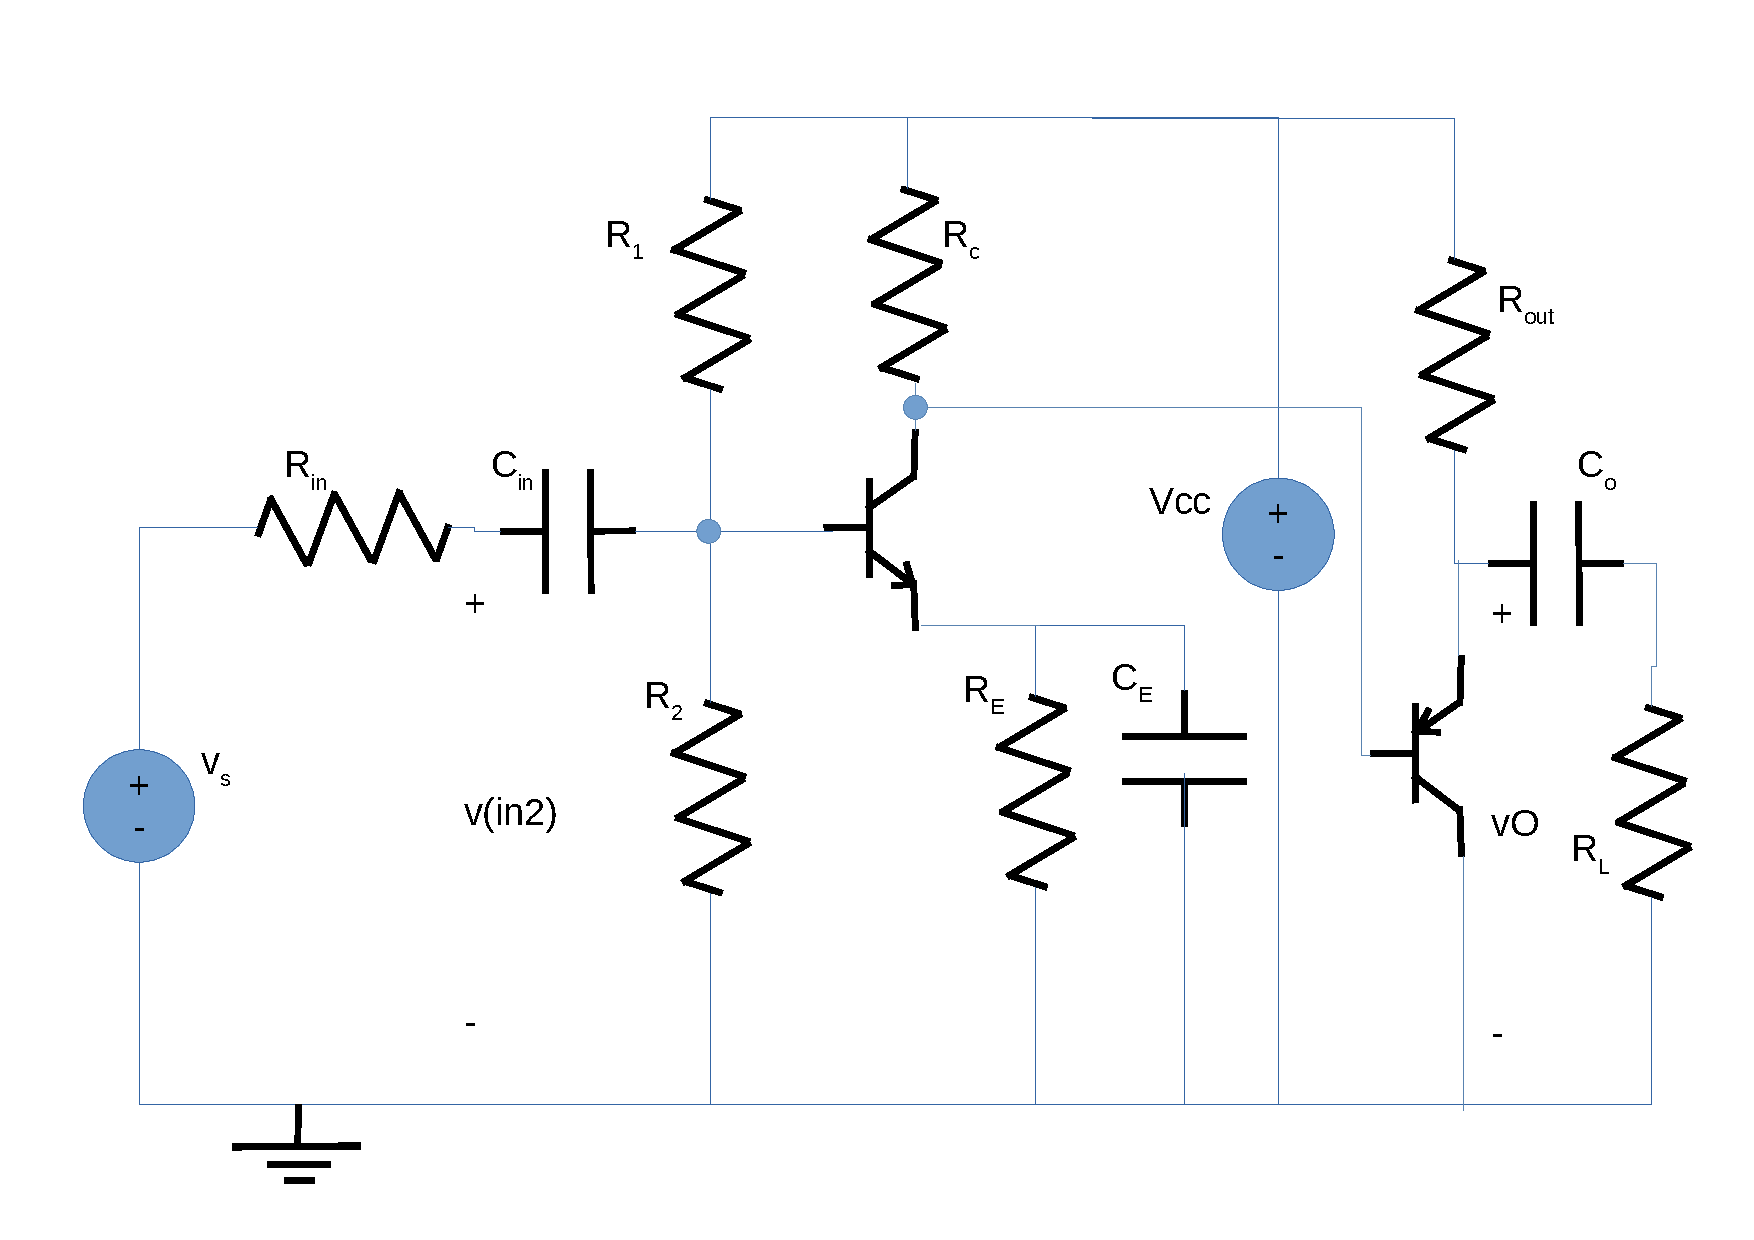
\includegraphics[width=1\linewidth]{circuitl4.pdf}
\caption{BJT Amplifier}
\label{fig:circuitol4}
\end{figure}

\clearpage
